\documentclass{article}
\usepackage{amsmath, amssymb}
\usepackage[retainorgcmds]{IEEEtrantools}
\usepackage{filecontents}
\usepackage{hyperref}
\usepackage{algpseudocode}
\author{Derek Kuo, Henry Milner}
\title{CS267 HW3}
\date{04/03/15}

% Some functions for general use.

\def\seqn#1\eeqn{\begin{align}#1\end{align}}

\newcommand{\vecName}[1]%
  {\boldsymbol{#1}}

\newcommand{\io}%
  {\text{ i.o. }}

\newcommand{\eventually}%
  {\text{ eventually }}

\newcommand{\tr}%
  {\text{tr}}

\newcommand{\Cov}%
  {\text{Cov}}

\newcommand{\adj}%
  {\text{adj}}

\newcommand{\funcName}[1]%
  {\text{#1}}

\newcommand{\hasDist}%
  {\sim}

\DeclareMathOperator*{\E}%
  {\mathbb{E}}

\newcommand{\Var}%
  {\text{Var}}

\newcommand{\std}%
  {\text{std}}

\newcommand{\grad}%
  {\nabla}

\DeclareMathOperator*{\argmin}{arg\,min}

\DeclareMathOperator*{\argmax}{arg\,max}

\newcommand{\inprod}[2]%
  {\langle #1, #2 \rangle}

\newcommand{\dd}[1]%
  {\frac{\delta}{\delta#1}}

\newcommand{\Reals}%
  {\mathbb{R}}

\newcommand{\indep}%
  {\protect\mathpalette{\protect\independenT}{\perp}} \def\independenT#1#2{\mathrel{\rlap{$#1#2$}\mkern2mu{#1#2}}}

\newcommand{\defeq}%
  {\buildrel\triangle\over =}

\newcommand{\defn}[1]%
  {\emph{Definition: #1}\\}

\newcommand{\example}[1]%
  {\emph{Example: #1}\\}

\newcommand{\figref}[1]%
  {\figurename~\ref{#1}}

\newtheorem{theorem}{Theorem}[section]
\newtheorem{lemma}[theorem]{Lemma}
\newenvironment{proof}[1][Proof]{\begin{trivlist}
\item[\hskip \labelsep {\bfseries #1}]}{\end{trivlist}}

\begin{filecontents}{\jobname.bib}
@inproceedings{shet2009asynchronous,
  title={Asynchronous programming in UPC: A case study and potential for improvement},
  author={Shet, Aniruddha and Tipparaju, Vinod and Harrison, Robert},
  organization={Citeseer}
}
\end{filecontents}

\begin{document}
\maketitle

\section{Introduction}
We first describe our implementation of distributed contig generation in UPC.  Then, we present some information about the performance and scaling properties of our implementation.  Finally, we offer some comments.

\subsection{Notation}
We use $P$ to denote the number of processors used in a computation.  We use $n$ to denote the number of kmers in a workload.  $H$ denotes the size of the hash table we use to store the kmers, which is always a multiple of $P$ (in fact it is equal to $P \operatorname{ceil}(n/P)$ in our experiments).  The hash value of a kmer is a number in the set $[H]$.  The ``local hash value'' of a kmer is its hash value modulo $H/P$.  The ``destination processor'' of a kmer is its hash value module $P$.

\section{Implementation}
A parallel implementation of contig generation is useful only for handling large genomes that grow with the problem size.  If we are sequencing genomes of a small fixed size, we have an embarrassingly parallel problem to which serial code is likely better suited.  So, when there are design choices to be made, we will target the large-genome regime.

\subsection{Graph Creation}
The hard part of graph creation is just a distributed hash-based shuffle, like the shuffle stage in a MapReduce job.  This involves all-to-all communication of approximately $1-1/P$ of the data.  Importantly, viewing graph creation as a hash shuffle means that we can a very small number of communication rounds, incurring network latency costs of only $O(P)$ rounds per processor and, as we will see, entirely avoiding the use of locks.

We partition the hash space evenly among processors, with processor $i$ receiving all kmers with hash value $\{iH/P, iH/P+1, \cdots, (i+1)H/P-1\}$.  Each processor reads a portion of the input file, then hashes each kmer to determine its destination processor.  Each processor writes the number of kmers it will send to each other processor (including itself), using a shared array of size $P^2$.  Then, for each processor $i$, for each other processor $j$, processor $i$ allocates a shared array with local affinity (a \texttt{shared [] kmer\_t *}, which we call a ``send buffer'') and places the kmers read on $i$ with destination processor $j$ in that send buffer.  (Shared pointers to these send buffers are placed in a shared array of size $P^2$.)  Then, after a single barrier, each processor allocates a private buffer to receive kmers from each other processor, and reads from the send buffers.

After each kmer has been shuffled to the appropriate machine, graph creation is embarrassingly parallel.  We create a shared array for the hash table, which is a \texttt{shared [1] shared\_kmer\_bucket\_t *} of size equal to the hash table size, where \texttt{shared\_kmer\_bucket\_t} is a \texttt{shared [] kmer\_t *}.  A kmer with destination processor $j$ and local hash value $h$ will reside in bucket $hP+j$ in this shared array.  Buckets are implemented as flat arrays; there is an additional shared array, a \texttt{shared [1] int *} of size equal to the hash table size, called a bucket-size table, to store the size of each bucket.  We first insert all the local kmers into temporary buckets that are private dynamic arrays, then allocate each bucket in shared memory with an appropriate size (with local affinity) and store its pointer in the shared hash table and its size in the shared bucket-size table.

In this scheme, a lookup in the hash table involves a lookup in the bucket-size table, a lookup in the hash table for a pointer to the bucket, and a \texttt{upc_memget} to fetch the bucket, which is of expected size $1$ (and maximum size $O(\log n / \log \log n)$ with high probability).  In our implementation, each of these steps is done serially, so there are $3$ rounds of communication for every lookup.

A few final notes on graph creation:
\begin{enumerate}
  \item All communication is done using packed kmers.  A packed kmer uses 2 bits per base pair, plus a byte to store its forward and backward extensions (which may be the usual nucleotides or the indicator for the start of a contig).
  \item It is possible in principle to pipeline the communication stage of the hash shuffle -- that is, each processor could communicate with each other processor simultaneously.  With full bisection bandwidth this would dramatically speed up the communication stage.  However, the version of UPC we are using does not seem to support asynchronous remote reads, so each processor must communicate serially with each other processor in our implementation.  Apparently there is some work on extending UPC to allow asynchronous remote communication \cite{shet2009asynchronous}.
\end{enumerate}

% \begin{algorithmic}
% \State numThreads $\gets$ the number of threads
% \State totalSize $\gets$ the number of kmers
% \State kmersTable $\gets$ a shared hash table
% \State hashShuffle()
% \State // Now localKmers is a list of kmers for this thread to handle.
% \For{each thread $i$ and kmer $k$}
%   \State insert $k$ into kmersTable, an entirely local operation.
% \EndFor
%
% \Function{hashShuffle}{}
%   \State // buckets $i*\texttt{numThreads}$ through $(i+1)*\texttt{numThreads}-1$ are stored in thread $i$'s memory.
%   \State localBuckets $\gets$ new DynamicArray<PackedKmer>[numThreads*numThreads]
%   \For{each thread $i$ and each local kmer $k$}
%     \State localBuckets[$i*\texttt{numThreads}$ + (hash($k$) $\%$ numThreads)].add($k$)
%   \EndFor
%   \For{each thread $i$}
%     \State // The following can be implemented efficient with \texttt{upc\_all\_scatter}:
%     \State numKmersToReceive $\gets$ new int[numThreads]
%     \For{each thread $j$}
%       \State numKmersToReceive[$j$] $\gets$ localBuckets[$j*\texttt{numThreads}+i$].size()
%     \EndFor
%     localKmers = new PackedKmer[numKmersToReceive.sum()]
%     \For{each thread $j$}
%       \State copy localBuckets[$j*$numThreads$+i$] into localKmers
%       \State increment localKmers to point past the copied kmers
%     \EndFor
%   \EndFor
% \EndFunction
% \end{algorithmic}

\subsection{Graph Traversal}
Graph traversal is straightforward.  Each machine filters its own kmers to find those with an \'F\' backward extension.  Then, for each machine (in parallel), for each kmer in the start list, we traverse the graph until we reach a kmer with an \'F\' forward extension.  Since we are guaranteed that we start at the end of a connected component that is a chain, traversing the graph is simply traversing a linked list.  Given that the last $K$ nucleotides of the current contig (including the last forward extension) are string $x$, we look up $x$ in the hash table.  The forward extension of that string gives us one nucleotide to extend the contig, or tells us we are done with the contig.  Each step involves (as noted above) 3 rounds of communication, except in the rare case that $x$ happens to reside on the same processor as the start kmer.

\section{Results}
\subsection{Small experiment}

\begin{figure}
  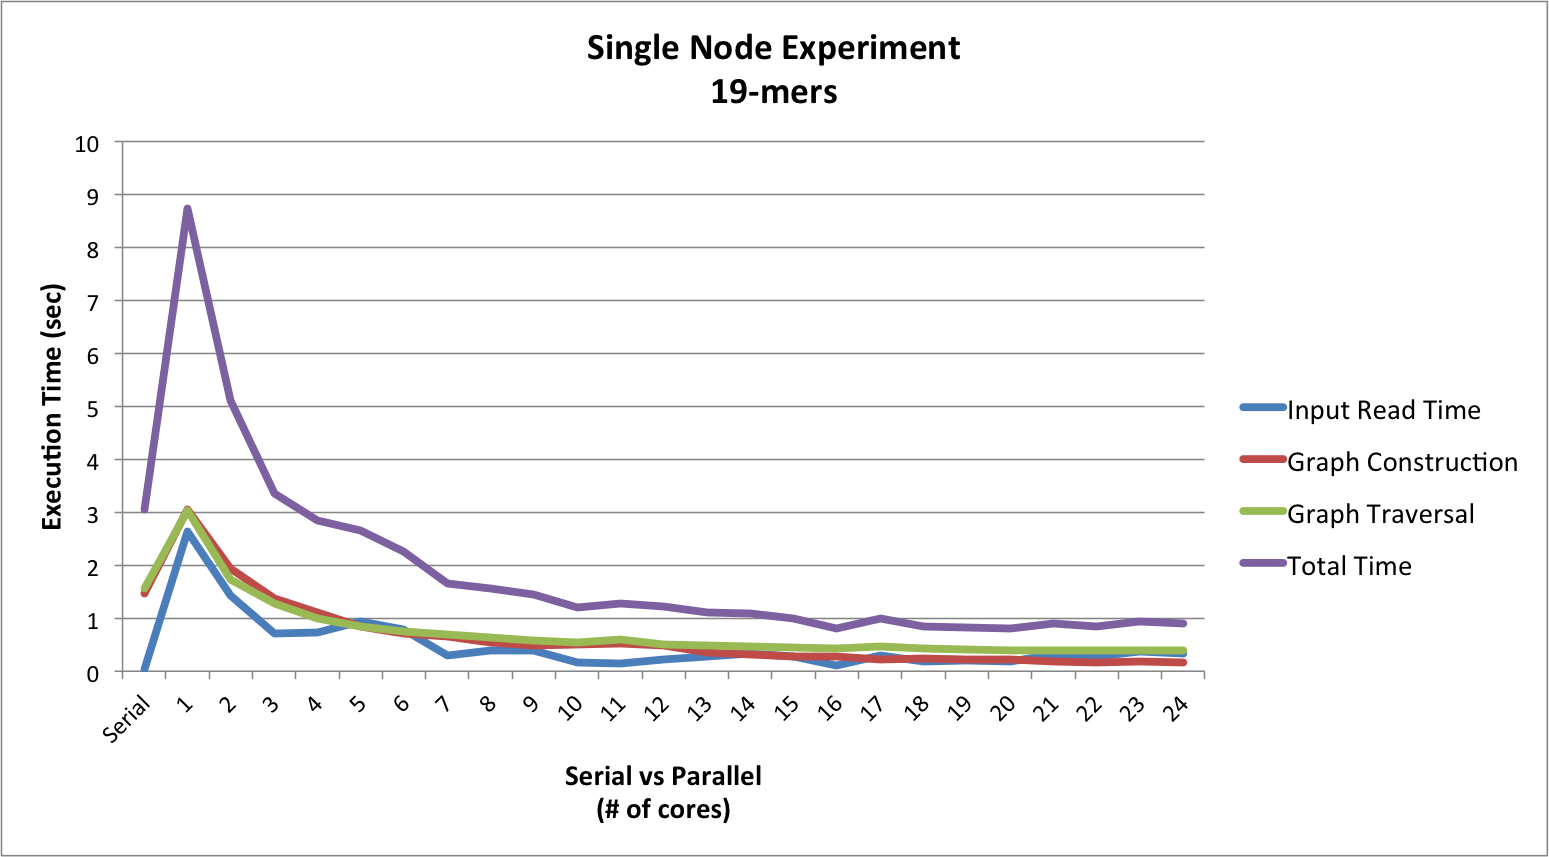
\includegraphics[width=\textwidth]{plots/Result_single_small.png}
  \caption{Comparison of serial and parallel algorithms on small input (19-mers).}
  \label{fig:all}
\end{figure}

When given a small 19-mers input, initially both graph construction and graph traversal functioned poorly on small core size (n<3). As the core size increased, we saw the performance of both algorithms improved continuously - Both construction and traversal execution time decreased, with construction time slightly outperformed traversal time.
\subsection{Large experiment}

\begin{figure}
  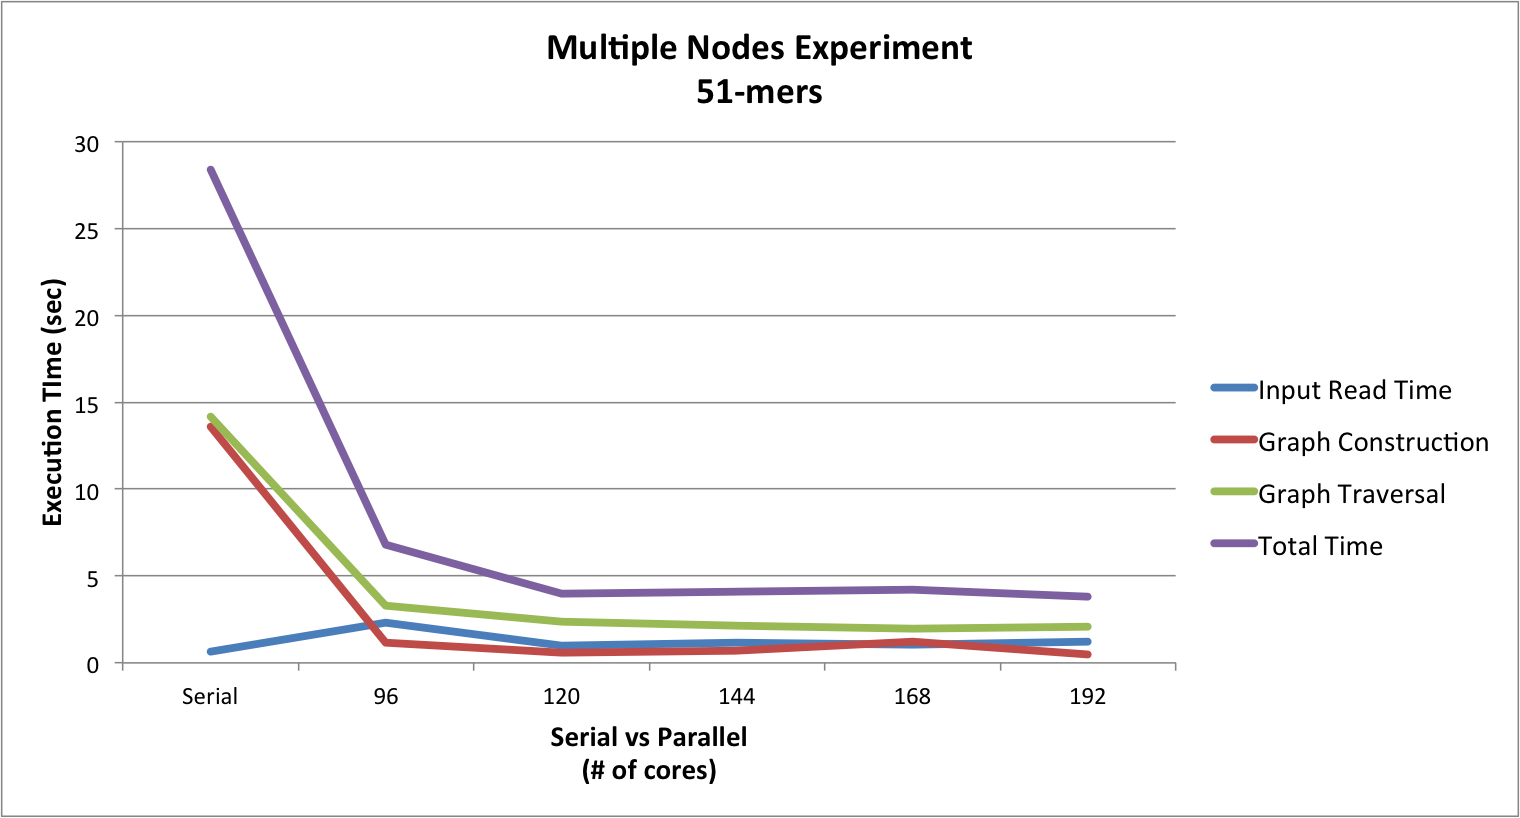
\includegraphics[width=\textwidth]{plots/Result_multiple_large.png}
  \caption{Comparison of serial and parallel algorithms on large input (51-mers).}
  \label{fig:all}
\end{figure}

For larger 51-mers input, the performance gap between serial de Bruijn algorithm and our parallel version became wider. All core sizes we tested (n=96,120,144,168,192) have at least 10 times faster on graph construction and 5 times faster on graph traversal. However, the performance between different core numbers didn't vary much for large core sizes (n>120), indicated that our algorithms can't scale up to improve performance further.    

\section{Discussion}
\subsection{Using UPC}
Programming with UPC for the first time was a surprisingly poor experience.  Our list of grievances is:
\begin{description}
  \item[No dynamic block size:] When using \texttt{upc\_all\_alloc}, it is never correct to use a block size that cannot be determined at compilation time, since the block size of the resulting pointer is a compile-time constant.  The UPC documentation never explicitly mentions this.
  \item[Misleading return type of \texttt{upc\_alloc}:] \texttt{upc\_alloc} returns a \texttt{shared void *}, but it is never correct to use it without casting it to a \texttt{shared [] void *}, since it has local affinity.  The UPC documentation never mentions this.
  \item[Poor standards support:] BUPC does not even support the C99 standard.  In particular, we would have liked to have support for dynamic-sized arrays on the stack.
  \item[Cryptic error messages:] Misuse of a shared pointer (see below) would result in a floating point exception in PGAS.  It would have been helpful to get a message like: ``This probably resulted from misuse of a shared pointer.''
  \item[Unclear shared pointer semantics:] We at first attempted to use the following scheme for our shared hash table: Each bucket was a linked list head, a struct holding both a kmer and a pointer to the next kmer (that is, a \emph{private} pointer into a \texttt{shared [] kmer\_t} on the machine owning the bucket).  Dereferencing the pointer on another machine did not work and resulted in a FPE.  In a rush to finish the project in time, we gave up on the linked-list scheme.  In retrospect, the problem was probably that we did not declare the pointer itself as shared within the struct.  However, it was not clear to us from the documentation that a private pointer-to-shared would not function properly if used on another processor.
  \item[No support for asynchronous remote communication:] As noted above, this slowed down our algorithm somewhat.
  \item[Required use of statics:] Statics make functional style impossible and make code more difficult to reason about.  Forgetting that shared objects must be stored in static fields, we at first attempted to use functional style.  It would have been helpful if the compiler had warned us when we incorrectly returned a pointer-to-shared from a function.
\end{description}

Some of these issues will be less painful if we use UPC a second time.  Many of our problems stemmed from thinking of UPC as providing a shared memory abstraction.  Given the large number of gotchas in dealing with shared memory, we think the value of UPC is in abstracting away the details of communication, rather than providing a real shared memory abstraction -- UPC is a slightly higher-level MPI.

\subsection{Implementation on Alternative Frameworks}
The hash-based shuffle described above would be easy to implement in MPI; it would probably look more natural. %FIXME

\subsection{Alternative Algorithms and Extensions}
Our implementation of graph creation seems close to optimal, given the requirement that the graph be partitioned among all available processors.  However, it is not clear that partitioning the graph is the best way to do graph traversal for contig generation.  If each processor (or at least each machine) has a local copy of the graph, and the number of contigs is large, the problem is embarrassingly parallel; the shared memory is only read during the traversal, never modified.  The only reason to introduce network communication into the algorithm is that the graph cannot fit into local memory that supports random accesses faster than network communication.  Using SSDs to store the graph on every machine (for example, Amazon EC2's \texttt{i2.8xlarge} instances) could be a superior alternative, and it would be unnecessary to use UPC.  If the data were initially distributed across machines, it would be important to use an efficient broadcast algorithm to send every kmer to every machine.

%FIXME: Talk about how the algorithm is like the distributed BFS algorithm.  If contigs were very long we'd have to use the traversal-stitching approach mentioned in lecture.

%\bibliographystyle{plain}
%\bibliography{\jobname}

\end{document}